\chapter{Podział metod tworzenia tablic sufiksów}

Tablice sufiksów zostały przedstawione w~roku 1990 przez Udiego Manbera i~Gene'a
Mayersa wraz z~pierwszym algorytmem ich tworzenia \cite{Manber90}.
Zestawienie ważniejszych algorytmów tworzenia tablic sufiksów
znajduje się w~tabeli \ref{tab:alg}. Autorzy pracy \cite{taxonomy} podsumowują
obecny stan wiedzy na temat tworzenia tablic sufiksów w~trzech punktach:
\begin{itemize}
  \item istnieją algorytmy efektywne pamięciowo o~złożoności liniowo zależnej
  od długości wejścia, np. \emph{smaller-larger}, \emph{skew},
  \item istnieją algorytmy szybsze w~praktycznych zastosowaniach pomimo swojej
  nieliniowej pesymistycznej złożoności, np. \emph{bpr}, \emph{improved  two-stage}, \emph{deep shallow}.
  \item każdy problem, którego rozwiązanie można znaleźć z~pomocą drzew sufiksów
  może zostać rozwiązany w~tym samym czasie przy pomocy tablic sufiksów
  \cite{replacing}.
\end{itemize}

\noindent
Niezrealizowanym do tej pory celem jest zaprojektowanie takiego algorytmu
tworzenia tablic sufiksów, który (za \cite{taxonomy}):
\begin{itemize}
  \item posiada minimalną złożoność asymptotyczną $\Theta(n)$,
  \item  jest szybki \emph{w~praktyce}, to znaczy na dużych rzeczywistych
  zbiorach danych, np. [\ref{hart}],
  \item jest \emph{lekki} -- wymaga niewiele więcej pamięci ponad ilość
  potrzebną do przechowania $x$ i~\SA{x}.
\end{itemize}


\noindent 
Autorzy prac \cite{taxonomy} oraz \cite{schurmann-phd} podjęli próbę stworzenia taksonomii
metod tworzenia tablic sufiksów. Proponowane przez nich metody są do siebie bardzo podobne,
a~klasyfikacja proponowana przez \cite{taxonomy} została rozbudowana w~pracy \cite{schurmann-phd}.
  
W~dalszej części pracy omówiona zostanie klasyfikacja proponowana przez Klausa-Bernda Schürmanna
\cite{schurmann-phd} poszerzona o~algorytm \emph{improved two-stage}.

\begin{table}[t]
	\begin{center}        
    \begin{tabular}{l c c c }
    \toprule
    Algorytm                  &           Publikacja            &    Złożoność obliczeniowa    & Złożoność pamięciowa \\ \midrule
    \emph{bpr}                &      \cite{schurmann-phd}       & $\bigO (\frac{n^2}{\log n})$ &       $9-10n$        \\         
    \emph{cache}              &          \cite{seward}          &     $\bigO(n^2 \log n)$      &         $9n$         \\         
    \emph{copy}               &          \cite{seward}          &     $\bigO(n^2 \log n)$      &         $5n$         \\         
    \emph{deep shallow}       &            \cite{MF}            &     $\bigO(n^2 \log n)$      &         $5n$         \\         
    \emph{difference-cover}   &      \cite{Burkhardt2003}       &      $\bigO(n \log n)$       &        $5-6n$        \\         
    \emph{improved two-stage} &            \cite{MP}            &     $\bigO(n^2 \log n)$      &         $5n$         \\         
    \emph{odd-even}           & \cite{kim} i~\cite{kim-jo-park} &    $\bigO(n \log \log n)$    &          --          \\         
    \emph{prefix-doubling}    &         \cite{Manber90}         &       $\bigO(n\log n)$       &         $8n$         \\         
    \emph{qsufsort}           &            \cite{LS}            &       $\bigO(n\log n)$       &         $8n$         \\         
    \emph{skew}               &            \cite{KS}            &          $\bigO(n)$          &       $10-13n$       \\         
    \emph{smaller-larger}     &          \cite{Ko2005}          &          $\bigO(n)$          &       $7-10n$        \\         
    \emph{two-stage}          &            \cite{IT}            &     $\bigO(n^2 \log n)$      &         $5n$         \\         
    \bottomrule
    \end{tabular}
    \end{center}                         
    \caption{Zestawienie ważniejszych metod tworzenia tablic sufiksów.
    Złożoność pamięciowa podana jest dla sytuacji, gdy jeden symbol zajmuje 1
    jednostkę pamięci a~jedna liczba -- 4 jednostki pamięci. Źródło: opracowanie
    własne na podstawie \cite{taxonomy} i~\cite{schurmann-phd}.}%
    \label{tab:alg}
\end{table}


\section{Podział metod ze względu na proces sortowania sufiksów}

W~pracy \cite{schurmann-phd} zaproponowano dwa ortogonalne typy klasyfikacji
algorytmów: pierwszy z~nich dzieli algorytmy ze względu na przebieg procesu
sortowania sufiksów; drugi ze
względu na sposób wykorzystania zależności między sufiksami. Podział
algorytmów według obu typów klasyfikacji przedstawiony jest w~tabeli
\ref{tab:schurmann}.

Klasyfikacja algorytmów ze względu na proces sortowania sufiksów opiera się na
odpowiedzi na pytanie: ,,które sufiksy są przetwarzane w~pierwszej kolejności
i~jak przebiega dalej proces sortowania?''. Algorytmy dzielone są następnie na 
dwie podgrupy: wykorzystujące \definicja{polepszanie kubełków} (\english{bucket
refinement}) oraz \definicja{sortowanie zredukowanych ciągów znaków} (\english{reduced string sorting}).


\subsection{Polepszanie kubełków}

Pod pojęciem polepszania kubełków kryje się utworzenie \emph{k-porządku}
sufiksów na podstawie wyliczonego wcześniej \emph{h-porządku} sufiksów ($k>h$).

Pierwszy typ algorytmów wykorzystujących polepszanie kubełków opiera się na ogólnych metodach
sortowania ciągów znaków (które nie wykorzystują wiedzy o~zależnościach między sufiksami). Algorytmy
tego typu wykonują \emph{h-sortowanie} dla zwiększającego się $h$ dopóki wszystkie \emph{h-grupy}
(kubełki) nie będą zawierały tylko jednego elementu. Algorytmy należące do tej kategorii to
\emph{MSD radix sort} omówiony w~pracy \cite{radix} i~\emph{multikey quicksort}
opisany~w~\cite{bentley}.

Drugi typ algorytmów polepszania kubełków opiera się na następującej obserwacji: jeżeli dwa sufiksy
słowa $x$ $x[u,n-1]$ i~$x[v,n-1]$ mają wspólny prefiks długości $\ell$, to ich porządek można
wywnioskować na podstawie porządku ich $\ell\textit{-następców}$ $x[u+\ell, n-1]$ i~$x[v+\ell, n-1]$
(przykładem tego procesu jest drugi etap algorytmu \emph{two-stage}). Algorytmy z~tej grupy można
podzielić na dwa dalsze podtypy:
\begin{itemize}
	\item algorytmy wykonujące \definicja{polepszanie wszerz}
	(\english{breadth-first refinement}). Metody te dokonują \emph{h-sortowania}
	ze zwiększającym się $h$~aż do uzyskania jednoelementowych kubełków
	(\emph{h-grup}). Do tej grupy algorytmów należą \emph{prefix-doubling} 
	\cite{Manber90} i~\emph{qsufsort} \cite{LS}.
	
	\item algorytmy wykonujące \definicja{polepszanie wgłąb} (\english{depth-first
	refinement}).
	Metody te wykorzystują następujący schemat polepszania kubełków: dla dowolnego
	$h$, sortowanie sufiksów kolejnego kubełka następuje dopiero po tym, gdy
	poprzedni kubełek jest w~pełni posortowany, czyli wszystkie jego podkubełki są
	jednoelementowe. Na przykład, dla ciągu ,,,AAABBABBBAAABBAB'' po
	\emph{1-sortowaniu} grupa sufiksów rozpoczynających się od symbolu $B$ będzie
	sortowana dopiero wtedy, gdy będzie ustalony porządek sufiksów
	rozpoczynających się od $A$; podczas sortowania tej grupy porządek sufiksów
	o~prefiksie ,,AB'' będzie ustalony dopiero po posortowaniu sufiksów rozpoczynających się od ,,AA'' itd.
	 Metody tego typu wykorzystują naiwne metody typu pierwszego w~sytuacji, 
	 gdy porządek $\ell\textit{-następców}$ jest jeszcze nieznany.
	 Do tej kategorii algorytmów należą między innymi: \emph{two-stage}, \emph{copy},
	  \emph{cache} oraz \emph{deep shallow}. W~ogólności metody tego typu są bardzo szybkie w~praktyce, pomimo ich wysokiej złożoności sięgającej nawet $\bigO(n^2\log n)$.
\end{itemize}

Rysunek \ref{rys:bucket-refinement} przedstawia etapy procesu polepszania
kubełków dla ciągu ,,AAABBABBBAAABBAB''. Każdy sufiks reprezentowany jest przez
pionową linię której wysokość oznacza jego pozycję według porządku
leksykograficznego: niska linia oznacza sufiks leksykograficznie mniejszy od
sufiksu reprezentowanego przez wyższą linię. Na rysunku
\ref{rys:bucket-refinement} widać (od góry): stan początkowy, stan w~trakcie
działania algorytmu (w przypadku polepszania wszerz jest to stan po
posortowaniu według prefiksu długości 2; dla polepszania wgłąb jest to stan po uporządkowaniu
sufiksów rozpoczynających się od symbolu ,,A''), stan końcowy -- posortowane sufiksy.

\begin{figure}[t]
    \begin{center}
        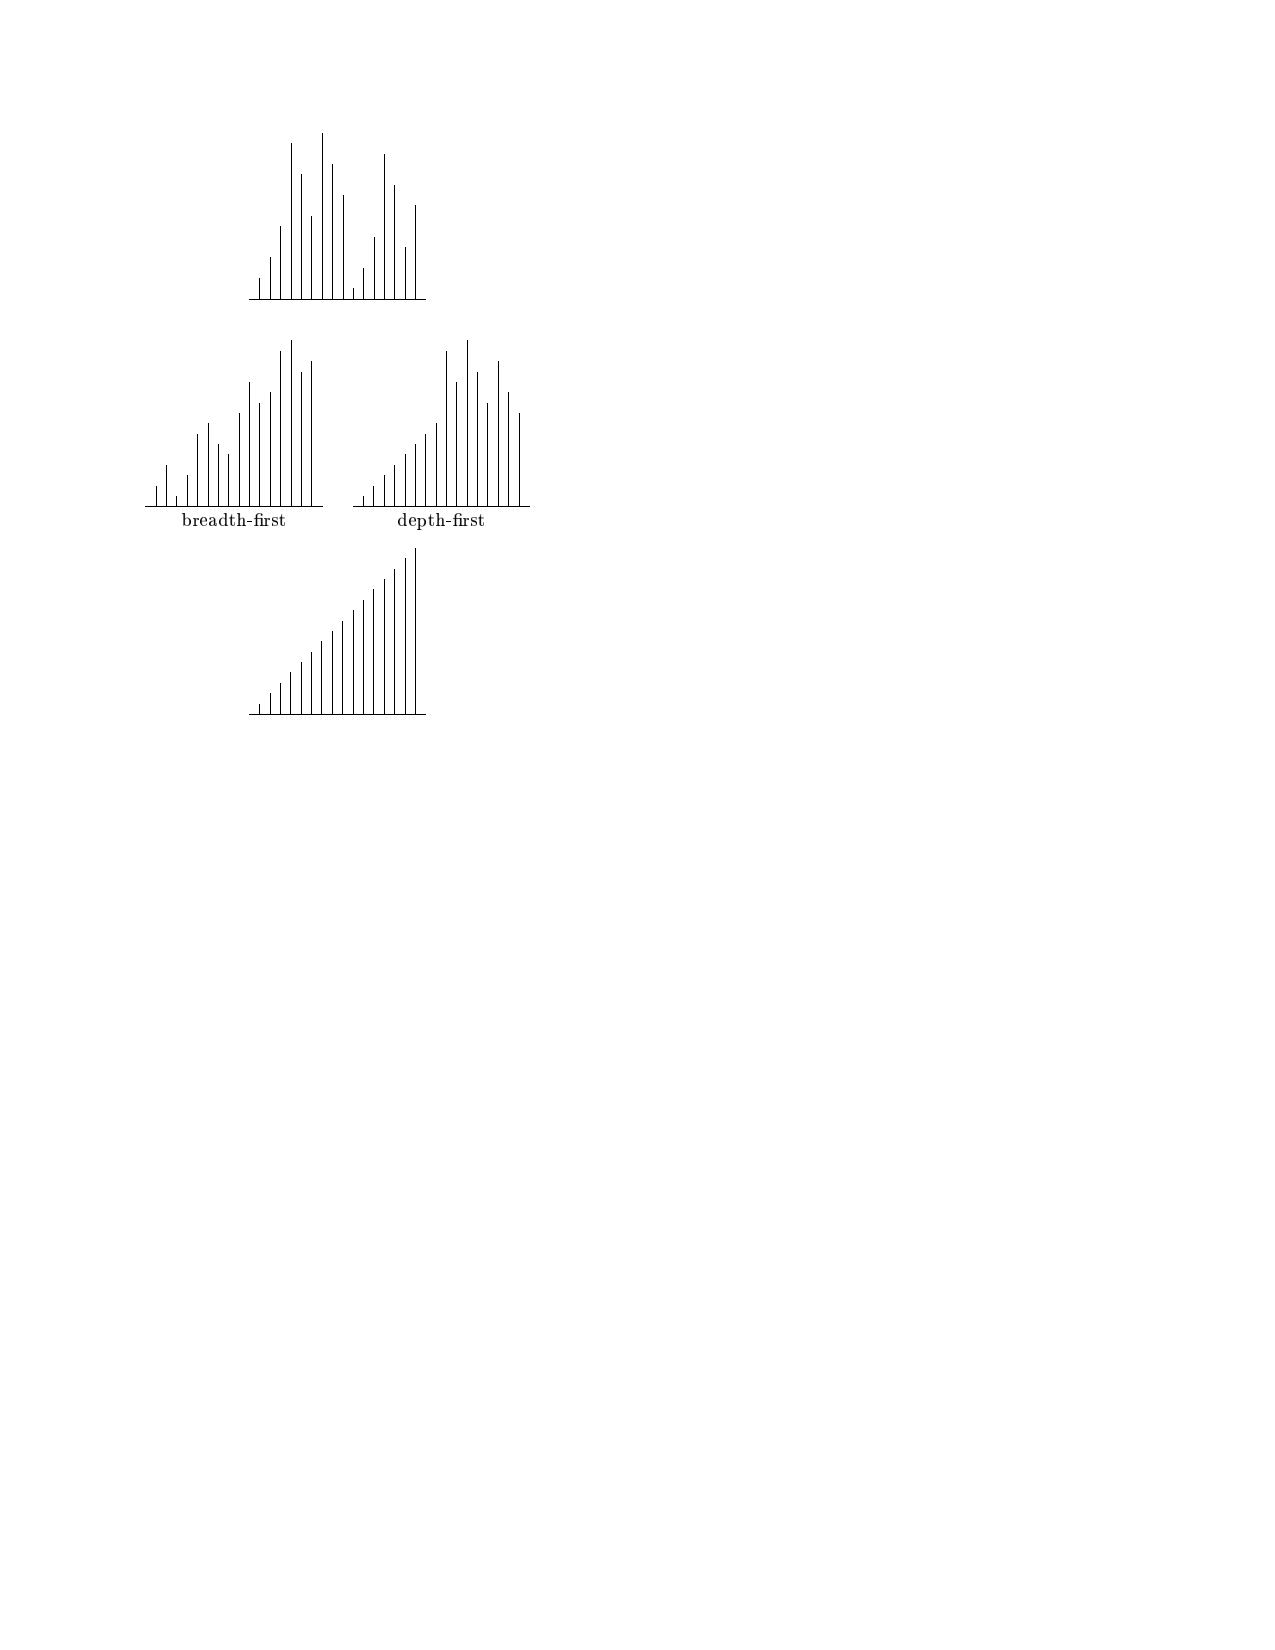
\includegraphics[scale=0.75]{figures/bucket-refinement.pdf}
    \end{center}        

    \caption{Etapy algorytmu polepszania kubełków dla wyrazu
    ,,AAABBABBBAAABBAB''. Źródło: \cite{schurmann-phd}.}%
    \label{rys:bucket-refinement}
\end{figure} 


\begin{table}[t]
	\begin{center}
    \begin{tabular}{l @{\hspace{2em}} c @{\hspace{2em}} c}
    \toprule
    Typ algorytmu            &     strategia \emph{push}             &    strategia \emph{pull}      \\
    \midrule
    Polepszanie wszerz       &        \emph{prefix-doubling}         &        \emph{qsufsort}        \\                                      
    \addlinespace[1em]
    Polepszanie wgłąb        &           \emph{two-stage}            &         \emph{cache}          \\                                      
                             &              \emph{copy}              &          \emph{bpr}           \\                                      
                             &          \emph{deep-shallow}          &                               \\                                      
                             &       \emph{improved two-stage}       &                               \\                                      
    \addlinespace[1em]
    Sortowanie zred.~ciągów znaków &        \emph{skew}              &    \emph{difference-cover}    \\                                      
                             &            \emph{odd-even}            &                               \\                                      
                             &         \emph{smaller-larger}         &                               \\                                      
    \bottomrule
    \end{tabular}
    \end{center}                         
    \caption{Podział algorytmów tworzenia tablic sufiksów według taksonomii
    zaproponowanej w~pracy \cite{schurmann-phd}. Źródło: opracowanie własne w~oparciu o~\cite{schurmann-phd}.}%
    \label{tab:schurmann}
\end{table}

\subsection{Sortowanie zredukowanych ciągów znaków}

Metody tego typu działają według następującego schematu: na początku wybierany jest podzbiór
\emph{sub} identyfikatorów sufiksów, odpowiadające im sufiksy są potem sortowane na podstawie
prefiksów ustalonej długości. Następnie każdemu z~tych sufiksów przypisywany jest pewien klucz
odpowiadający jego porządkowi wg. prefiksów. Następnie tworzony jest taki ciąg $t^{\textit{sub}}$
długości $|\textit{sub}|$ zawierający wcześniej przydzielone klucze, którego \SA{t^{\textit{sub}}}
odpowiada porządkowi leksykograficznemu sufiksów identyfikowanych zbiorem \emph{sub}. Tablica
\SA{t^{\textit{sub}}} może być obliczana rekurencyjnie tym samym algorytmem, lub z~wykorzystaniem
efektywnego algorytmu sortowania ciągów znaków (\cite{bentley-sort}, \cite{radix}, [\ref{ssort}],
\cite{bentley}, \cite{sinha}). W~pełni uporządkowane sufiksy ze zbioru \emph{sub} służą potem do
posortowania pozostałych sufiksów. Ostatecznie budowana jest pełna tablica sufiksów. Do algorytmów
realizujących powyższy schemat należą: \emph{difference-cover}, \emph{skew}, \emph{odd-even} oraz
\emph{smaller-larger}.

Rysunek \ref{rys:reduced-string-sorting} przedstawia etapy działania algorytmu
sortowania zredukowanych ciągów znaków. Podobnie jak na rysunku
\ref{rys:bucket-refinement}, sufiksy reprezentowane są przez pionowe linie,
których wysokość oznacza miejsce sufiksu w~porządku leksykograficznym. Sufiks
reprezentowany przez mniejszą linię jest leksykograficznie mniejszy od sufiksu
reprezentowanego przez wyższą linię. Na rysunku przedstawiono po kolei (od
góry): stan początkowy; stan algorytmu w~sytuacji gdy posortowane są sufiksy
o~nieparzystych identyfikatorach; stan końcowy.


\begin{figure}[t]
    \begin{center}
        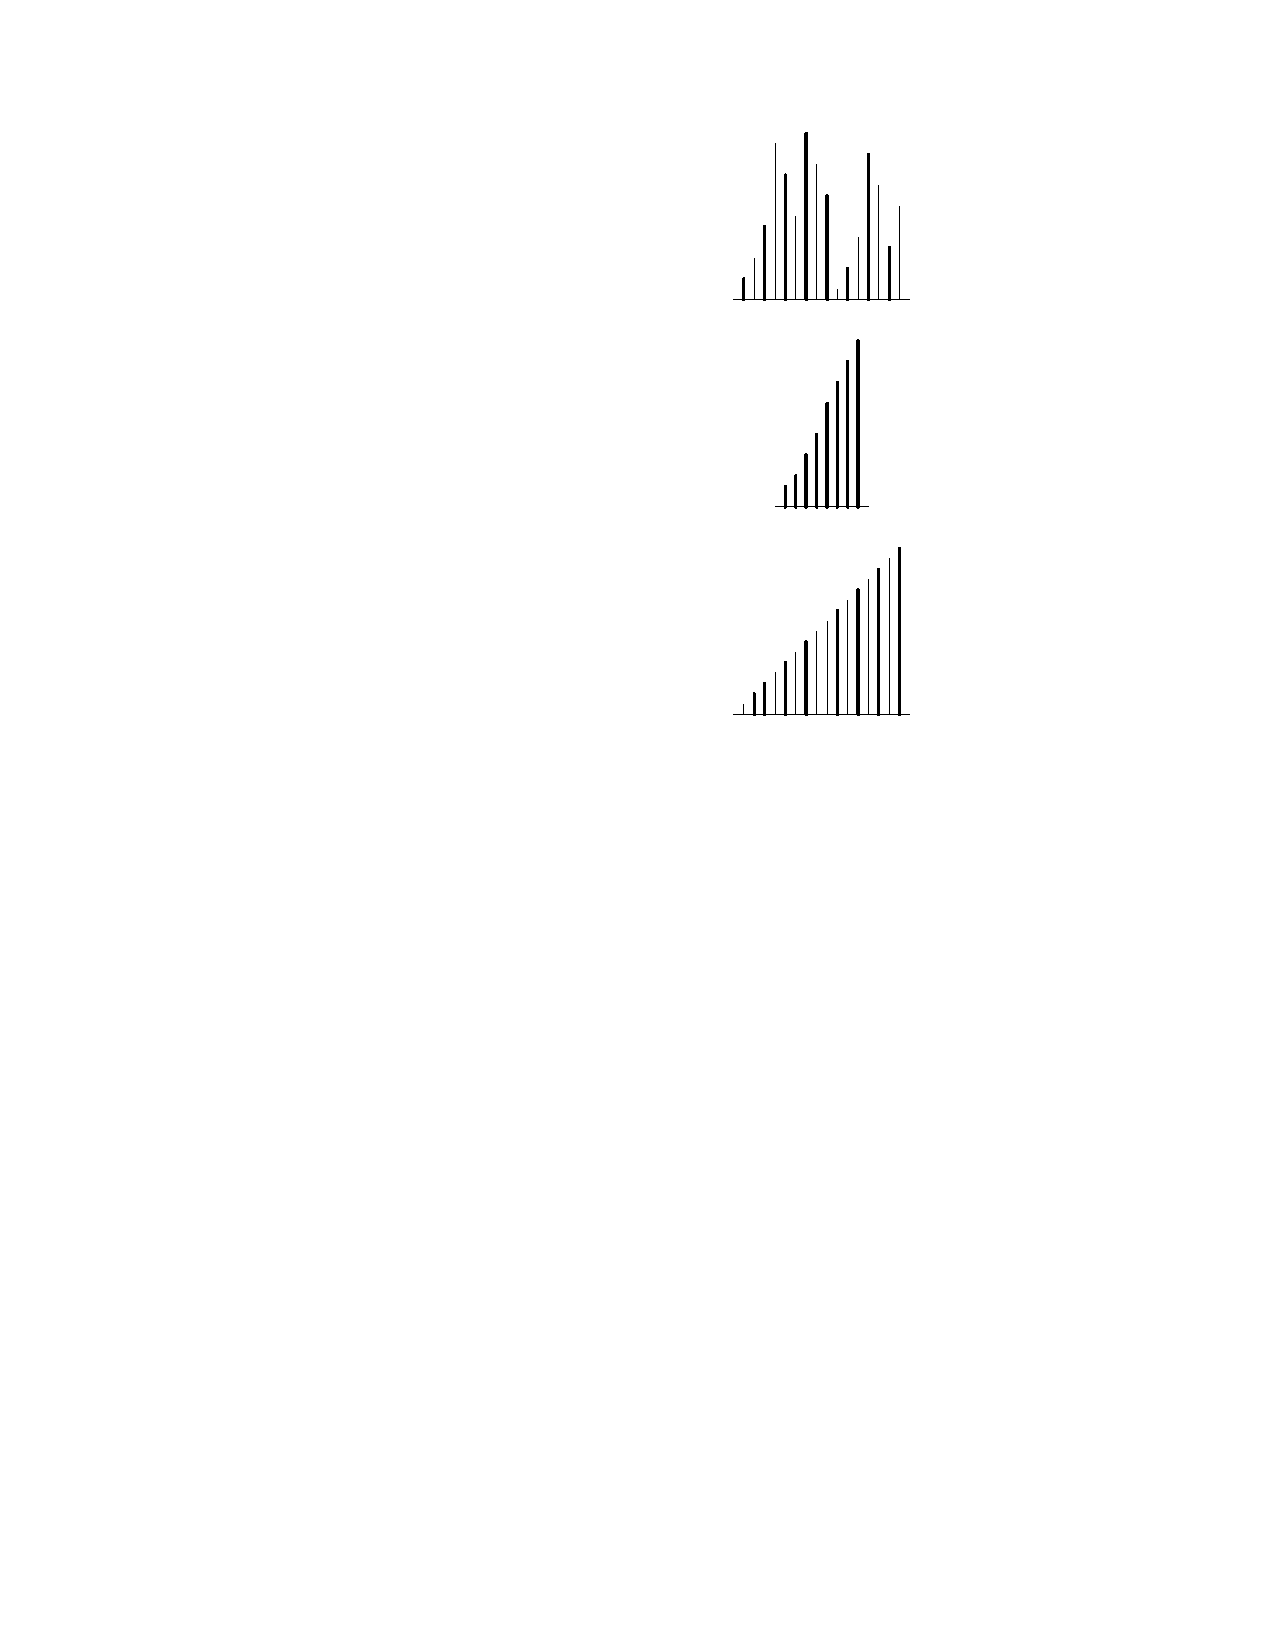
\includegraphics[scale=0.75]{figures/reduced-string-sorting.pdf}
    \end{center}        
    \caption{Etapy algorytmu sortowania zredukowanych ciągów znaków dla wyrazu
    ,,AAABBABBBAAABBAB''. Źródło: \cite{schurmann-phd}.}%
    \label{rys:reduced-string-sorting}
\end{figure} 

\section{Podział ze względu na sposób wykorzystania zależności między sufiksami}

Drugim sposobem podziału zaproponowanym w~pracy \cite{schurmann-phd} jest
podział algorytmów tworzenia tablic sufiksów ze względu na sposób wykorzystania
zależności między sufiksami. Jeżeli dwa sufiksy $x[u,n-1]$ i~$x[v,n-1]$ mają
wspólny prefiks długości $\ell$, to ich porządek można ustalić na podstawie
porządku sufiksów $x[u+\ell,n-1]$ i~$x[v+\ell,n-1]$. Rozróżnia się dwie metody
wykorzystywania tej zależności: metodę \emph{pull} i~metodę
\emph{push}.
Terminy \emph{pull} i~\emph{push} pochodzą z~terminologii systemów
informacyjnych, oznaczają różne strategie komunikacji pomiędzy nadawcą
wiadomości i~jej odbiorcą. Metoda \emph{push} oznacza sytuację, kiedy dostawca
wiadomości nawiązuje komunikację. Odwrotna sytuacja następuje w~strategii
\emph{pull} -- tutaj to odbiorca zgłasza żądanie inicjalizacji komunikacji.

W~odniesieniu do algorytmów tworzenia tablic sufiksów metoda \emph{push} polega na tym, że
wykorzystuje porządek wcześniej obliczonych grup sufiksów do ustalenia porządku grup sufiksów
$\ell$\textit{-poprze\-dni\-ków}, tzn. po ustaleniu porządku sufiksów $x[u+\ell,n-1]$ i~$x[v+\ell,n-1]$
obliczany jest porządek sufiksów $x[u,n-1]$ i~$x[v,n-1]$. Wzorcowym przykładem wykorzystania tej
techniki jest algorytm \emph{two-stage}.

Metoda \emph{pull} jest wykorzystywana w~procesie sortowania opierającego się o~porównania. Podczas
porównywania sufiksów $x[u,n-1]$ i~$x[v,n-1]$ sprawdzany jest porządek sufiksów $x[u+\ell,n-1]$
i~$x[v+\ell,n-1]$. Algorytm \emph{qsufsort} jest najlepszym przykładem zastosowania tej techniki.

